\documentclass[
	% -- opções da classe memoir --
	article,			% indica que é um artigo acadêmico
	11pt,				% tamanho da fonte
	oneside,			% para impressão apenas no recto. Oposto a twoside
	a4paper,			% tamanho do papel. 
	% -- opções da classe abntex2 --
	%chapter=TITLE,		% títulos de capítulos convertidos em letras maiúsculas
	%section=TITLE,		% títulos de seções convertidos em letras maiúsculas
	%subsection=TITLE,	% títulos de subseções convertidos em letras maiúsculas
	%subsubsection=TITLE % títulos de subsubseções convertidos em letras maiúsculas
	% -- opções do pacote babel --
	english,			% idioma adicional para hifenização
	brazil,				% o último idioma é o principal do documento
	sumario=tradicional
	]{abntex2}


% ---
% PACOTES
% ---

% ---
% Pacotes fundamentais 
% ---
\usepackage{lmodern}			% Usa a fonte Latin Modern
\usepackage[T1]{fontenc}		% Selecao de codigos de fonte.
\usepackage[utf8]{inputenc}		% Codificacao do documento (conversão automática dos acentos)
\usepackage{indentfirst}		% Indenta o primeiro parágrafo de cada seção.
\usepackage{nomencl} 			% Lista de simbolos
\usepackage{color}				% Controle das cores
\usepackage{graphicx}			% Inclusão de gráficos
\usepackage{microtype} 			% para melhorias de justificação
% ---
		
% ---
% Pacotes adicionais, usados apenas no âmbito do Modelo Canônico do abnteX2
% ---
\usepackage{lipsum}				% para geração de dummy text
% ---
		
% ---
% Pacotes de citações
% ---
\usepackage[brazilian,hyperpageref]{backref}	 % Paginas com as citações na bibl
\usepackage[alf]{abntex2cite}	% Citações padrão ABNT

\usepackage{backnaur} %  especificação da grmática
\usepackage{syntax} % especificação gramática
\usepackage{subfiles} % modularização em arquivos
\usepackage{hyperref} % hyper-links

%%%%%%%%%%%%%%%%%%%
%%%%%%%%%%%%%%%%%%% https://tex.stackexchange.com/questions/348651/c-code-to-add-in-the-document
%%%%%%%%%%%%%%%%%%%
\usepackage{xcolor}
\usepackage{listings}		% Para as regras da gramatica
\usepackage{pxfonts}    % para deixar em negrito algumas partes da gramática
\usepackage{graphicx}   % imagens

%\lstset{
%	basicstyle=\ttfamily,
%	xleftmargin=3em,
%	literate={->}{$\rightarrow$}{2}
%	{α}{$\alpha$}{1}
%	{δ}{$\delta$}{1}
%}

\lstset{language=C,
	basicstyle=\ttfamily,
	keywordstyle=\bfseries,
	showstringspaces=false,
	texcl=<true|false>,
	morekeywords={ahead, SCAN, PRINT, ICAST, FCAST, mat, IREAD, FREAD, COPY}
}

\definecolor{mGreen}{rgb}{0,0.6,0}
\definecolor{mGray}{rgb}{0.5,0.5,0.5}
\definecolor{mPurple}{rgb}{0.58,0,0.82}
\definecolor{backgroundColour}{rgb}{0.95,0.95,0.92}

\lstdefinestyle{CStyle}{
	backgroundcolor=\color{backgroundColour},   
	commentstyle=\color{mGreen},
	keywordstyle=\color{magenta},
	numberstyle=\tiny\color{mGray},
	stringstyle=\color{mPurple},
	basicstyle=\footnotesize,
	breakatwhitespace=false,         
	breaklines=true,                 
	captionpos=b,                    
	keepspaces=true,                 
	numbers=left,                    
	numbersep=5pt,                  
	showspaces=false,                
	showstringspaces=false,
	showtabs=false,                  
	tabsize=2,
	language=C
}
%%%%%%%%%%%%%%%%%%%
%%%%%%%%%%%%%%%%%%%
%%%%%%%%%%%%%%%%%%%

% ---

% ---
% Configurações do pacote backref
% Usado sem a opção hyperpageref de backref

\renewcommand{\it}[1]{\textit{#1}}
\renewcommand{\bf}[1]{\textbf{#1}}

\renewcommand{\backrefpagesname}{Citado na(s) página(s):~}
% Texto padrão antes do número das páginas
\renewcommand{\backref}{}
% Define os textos da citação
\renewcommand*{\backrefalt}[4]{
	\ifcase #1 %
		Nenhuma citação no texto.%
	\or
		Citado na página #2.%
	\else
		Citado #1 vezes nas páginas #2.%
	\fi}%
% ---

% --- Informações de dados para CAPA e FOLHA DE ROSTO ---
\titulo{C-mat: um mini-C com matrizes}
%\tituloestrangeiro{Canonical article template in \abnTeX: optional foreign title}

\autor{
Leonardo Maffei da Silva\thanks{leoitu22hotmail.com@gmail.com. \url{https://www.linkedin.com/in/leonardo-maffei-ti/}} }

\local{Brasil}
\data{2019}
% ---

% ---
% Configurações de aparência do PDF final

% alterando o aspecto da cor azul
\definecolor{blue}{RGB}{41,5,195}

% informações do PDF
\makeatletter
\hypersetup{
     	%pagebackref=true,
		pdftitle={\@title}, 
		pdfauthor={\@author},
    	pdfsubject={Modelo de artigo científico com abnTeX2},
	    pdfcreator={LaTeX with abnTeX2},
		pdfkeywords={abnt}{latex}{abntex}{abntex2}{atigo científico}, 
		colorlinks=true,       		% false: boxed links; true: colored links
    	linkcolor=blue,          	% color of internal links
    	citecolor=blue,        		% color of links to bibliography
    	filecolor=magenta,      		% color of file links
		urlcolor=blue,
		bookmarksdepth=4
}
\makeatother
% --- 

% ---
% compila o indice
% ---
\makeindex
% ---

% ---
% Altera as margens padrões
% ---
\setlrmarginsandblock{3cm}{3cm}{*}
\setulmarginsandblock{3cm}{3cm}{*}
\checkandfixthelayout
% ---

% --- 
% Espaçamentos entre linhas e parágrafos 
% --- 

% O tamanho do parágrafo é dado por:
\setlength{\parindent}{1.3cm}

% Controle do espaçamento entre um parágrafo e outro:
\setlength{\parskip}{0.2cm}  % tente também \onelineskip

% Espaçamento simples
\SingleSpacing


% ----
% Início do documento
% ----
\begin{document}

% Seleciona o idioma do documento (conforme pacotes do babel)
%\selectlanguage{english}
\selectlanguage{brazil}

% Retira espaço extra obsoleto entre as frases.
\frenchspacing 

% ----------------------------------------------------------
% ELEMENTOS PRÉ-TEXTUAIS
% ----------------------------------------------------------

%---
%
% Se desejar escrever o artigo em duas colunas, descomente a linha abaixo
% e a linha com o texto ``FIM DE ARTIGO EM DUAS COLUNAS''.
% \twocolumn[    		% INICIO DE ARTIGO EM DUAS COLUNAS
%
%---

% página de titulo principal (obrigatório)
\maketitle


% titulo em outro idioma (opcional)



% resumo em português
\begin{resumoumacoluna}
 Este documento atende os fins de documentação da quarta
 parte do projeto final da disciplina \textit{Tradutores},
 ministrada pela professora Dr.a Cláudia Nalon, no segundo semestre de 2019, na Universidade de Brasília. Tal artefato descreve um pouco da implementação do analisador semântico, bem como dificuldades encontradas durante tal processo. Para esta fase novamente refez-se a gramática, a fim de reduzir a quantidade de regras e tratar alguns \it{bugs} presentes na antiga, e aproveitando o fato de que seria necessário a reimplementação completa do analisador sintático.
 \vspace{\onelineskip}
 
 \noindent
 \textbf{Palavras-chave}: C, linguagem, matriz, primitiva.
\end{resumoumacoluna}




\newcommand{\terminal}[1]{ \bnfpn{\textbf{#1}} }

\newcommand{\production}[1]{\bnfpn{\textit{#1}}}
\newcommand{\IT}[1]{\textit{#1}}
\newcommand{\BF}[1]{\textbf{#1}}

%\setlength{\grammarparsep}{20pt plus 1pt minus 1pt} % increase separation between rules
%\setlength{\grammarindent}{12em} % increase separation between LHS/RHS 

\section{Introdução}
Implementar-se-á, até a versão final deste artigo, um compilador para a linguagem proposta. Para sua realização, serão utilizados os conhecimentos adquiridos na disciplina \textit{Tradutores}, ministrada pela professora \hyperref{http://lattes.cnpq.br/7793795625581127}{}{}{Cláudia Nalon}.

\section{Usuário característico}
Destina-se ao estudante de álgebra linear, o qual pode usar a linguagem para, por exmeplo, confirmar se sua resolução de um sisema linear encontra-se correta, tudo isso de maneira rápida e eficiente.

\section{Motivação}
Durante a realização do curso de Cálculo Numérico, o grupo do autor notou a ausência dessa \it{feature} na linguagem C. Desse modo, foi necessária a simulação desse tipo de dados, à época implementada por meio de inúmeras funções. Se houvese um tipo nativo para matriz bem como operações elementares sobre seus elementos, teria sido de grande auxílio à codificação dos diversos métodos numéricos requeridos pela disciplina.
\par


\section{Gramática}

Para esta fase, a diferença mais marcante na gramática está na especificação de precedência de operadores não mais inerente à gramática (conforme fora feito nos trabalhos anteriores), mas sim por meio das diretivas \it{\%left} e \it{\%right} do \it{bison}. Além disso, novas \it{features} foram adicionadas à gramática, a saber:
\begin{itemize}
	\item declaração e inicialização de variáveis em apenas um \it{statement}
	\item não utilização da palavra reservada \bf{void} quando se define ou chama função sem parâmetros
	\item pode-se ter \bf{;} como \it{statement} local (desse modo, mais de um ponto e vírgula não causa erro)	
\end{itemize}
Foram também retiradas algumas coisas, quais sejam:
\begin{itemize}
	\item remoção dos tipo \bf{char} e \bf{void}
	\item remoção de regras que serviam como "demultiplexadoras dummy" de operadores
	\item declaração de variáveis deve vir antes dos demais \it{statements} de uma função
\end{itemize}
O tipo \bf{char} foi removido pois sua única função reside em servir de parâmetro à declaração \bf{PRINT}. Agora, existe mais esse tipo de dado, mas é possível a criação de \it{statements} utilizando diretamente o caractere desejado; por exemplo, \bf{PRINT('a')}.
Além das adições / remoções enumeradas, foi adicionada uma regra específica para declaração de variáveis, separada da declaração de parâmetros, além da possibilidade de explicitar que um parâmetro é um vetor.
A seguir, a especificação da nova gramática:
%% BEGIN GRAMÁTICA
	\subfile{grammar.tex}
%% END GRMÁTICA

As palavras reservadas da linguagem aparecem em \bf{negrito} na gramática, os outros \it{tokens} estão em letras maiúsculas e as regras de produção estão em letras minúsculas. Além As principais limitações de C-mat são listadas abaixo:
\begin{itemize}
	\item declaração de variáveis apenas no escopo local ou no início de funções
	\item matrizes são sempre bidimensionais
	\item vetores são unidimensionais e suportam apenas os tipos \bf{int} e \bf{float}
\end{itemize}
Essas limitações tem por objetivo simplificar a implementação do tradutor dado o período de apenas um semestre e são todas garantidas pela gramática da linguagem.
% ----------------------------------------------------------
% Introdução
% ----------------------------------------------------------


% ----------------------------------------------------------
% Seção de explicações
% ----------------------------------------------------------




\section{Semântica}
A principal mudança nessa nova fase do projeto está na impossibilidade de indexação de variáveis que não são vetores nem matrizes (ideia inicial do projeto). De resto, não houve grandes alterações. A semântica é em grande parte idêntica à da linguagem C, em especial nos pontos que possuem em comum (operações de adição, subtração, etc) e nos tipos básicos \it{int} e \it{float}. 

Construtos de controle de fluxo se comportam de maneira idêntica à de C, embora seja necessário que todo \it{statement} \it{if}/\it{else} seja seguido por um bloco de código. O construto \it{while} tem funcionamento idêntico em ambas as linguagens; operações de \it{cast} devem ser feitas por meio dos operadores \it{ICAST} e \it{FCAST}, mas caso não sejam utilizados e conversão ainda pode ser feita, embora seja emitido mensagem de aviso ao usuário.

Só é possível a realização de \it{cast} entre escalares (\bf{int} e \bf{float}); outras tentativas de conversão são caracterizadas como erros. C-mat possui apenas dois escopos: global e local. Caso uma variável utilizada dentro de uma função não tenha sido declarada, esta é buscada no escopo global. Caso não seja encontrada, é reportado erro. Não foi implementado o escopo de bloco com o
único intuito de facilitar a implementação da análise semântica. Um dos motivos foio débito relativo ao analisador sintático que para ser quitado requeriu, conforme citado em \ref{difSintatico}, o que tomou uma quantia significativa de tempo.

Operadores binários são e maneira geral associativos à esquerda, com exceção para o operador de potenciação de matriz \bf{@@}, visto que a operação de potenciação é associativa à direita tal qual na matemática usual. Há operadores para as seguintes operações:
\begin{itemize}
	\item adição/subtração
	\item multiplicação/divisão
	\item resto da divisão
	\item comparação (maior que, menor que, maior ou igual a, menor ou igual a, igual e não igual)
	\item AND e OR lógicos
	\item NOT lógico
	\item operador endereço (\&)
	\item multiplicação de matrizes
	\item exponenciação de matrizes
\end{itemize}

Todas as operações acima, a menos das relacionadas a matrizes, podem ser aplicadas a dois escalares quaisquer, embora caso esses operandos não sejam de mesmo tipo será mostrada mensagem de aviso ao usuário. Em caso de operação entre tipos distintos, feita a conversão de tipos: inteiros são convertidos para ponto flutuante na maioria dos casos, exceto quando trata-se do operador de resto da divisão, situação na qual o contrário ocorre. Operadores relacionais são um caso especial; quando aparecem, o resultado da operação é sempre um \bf{inteiro}: 0 ou 1. O operador \bf{!} nada mais faz do que troca o valor de seu operando 0 para 1 ou de qualquer outro valor para 1. Em caso de o valor ser um ponto flutuante, a conversão para inteiro é feita, e então seu efeito é aplicado ao valor convertido. Em qualquer outro caso, considera-se que houve um erro.

É possível definir a assinatura de uma função antes de sua definição por meio da estrutura \bf{ahead} BASE\_TYPE ID; contudo, isso só pode ser feito uma vez para cada nome de função (limitação que não limita o poder da funcionalidade, porém facilitou a implementação). Desse modo, pode-se efetuar checagem de tipo e de parâmetros de funções sem que seja necessário percorrer a árvore abstrata mais de uma vez, e portanto é possível a implementação em C-mat de recursão indireta.

Conforme entregas passadas, há vetor como tipo de dados composto; porém, não é possível ter vetores multidimensionais e só é possível a instanciação de vetores de escalares. Matrizes podem ser contruídas
enquanto tipos nativos da linguagem, em notação similar ao que seria um vetor bidimensional, porém com o
adicional de ser te informar qual o tipo escalar que a matriz armazena. Contudo, novamente por conta de
possíveis problemas na hora da tradução, C-mat implementa apenas \it{matrizes 2D}. Ainda assim,
acredita-se que grande parte dos problemas encontrados pelo usuário a que se destina C-mat não lidam com
matrizes com mais de duas dimensões e, portanto, essa limitação não deve ser um problema de maneira
geral.


\iffalse
\section{Exemplo de programa na linguagem}
A seguir, trechos de código pertencente à nova linguagem.

\begin{lstlisting}[style=CStyle]
int main() {
float a = 10.1;
float c = 10.;

mat int m[3][3] = [
	{1, 0, 0} 
	{0 ,1, 0} 
	, 0, 1}
];
READ(a);
\end{lstlisting}
\fi

\section{Implementação}
\label{implementacao}

Nesta fase houve pouca alteração no analisador léxico, pois o conjunto de tokens manteve-se praticamente o mesmo. A gramática por sua vez, bem como o analisador sintático, foram refeitos do zero, 
embora se tivesse em mente que a linguagem gerada pela gramática deveria ser bastante similar à que era gerada pela antiga. O analisador sintático teve de ser refeito pois a estrutura adotada 
anteriormente não era escalável, de difícil manutenção e número bastante alto de estruturas de dados \it{dummy}.

A nova implementação trata cada nó da árvore abstrata como uma estrutura de dados que é comum a todos eles, diferenciando-se pelo nome do token e outros atributos, sendo o principal sua entrada na tabela de símbolos (cada nó da AST correspondente a algum identificador possui um 
ponteiro para a entrada na tabela de símbolos que contém informações sobre si).

A estrutura de árvore é obtida fazendo-se cada nó relativo a uma cabeça de produção apontar para o primeiro de seus filhos, o qual juntamente com seus irmãos encadeia a lista de filhos da cabeça da regra. Ações semânticas são realizadas quase sempre ao final da redução de uma regra; exceções a este padrão
são encontradas na regras de declaração e definição de função bem como na regra que gera chamada de função, ações essas que setam a variável cujo valor é o escopo atual ou verificam se um
identificador representa mesmo uma função.

A análise semântica é realizada juntamente com a montagem da árvore abstrata, sem necessidade de percorrê-la mais de uma vez (exceção para a checagem de assinatura de chamada e definição de função). Logo, é feita em \it{apenas uma passada}. Tal decisão foi tomada pois previu-se que a análise em mais de um passada seria bastante trabalhosa e não traria benefícios significativos (o principal
benefício seria a possibilidade de recursão indireta; porém, para resolução desse problema, C-mat permite a declaração de função antes de sua utilização).

\subsubsection{Limitações}

Primeiramenre, ressalte-se que boa parte da análise semântica foi realizada com sucesso; contudo, há algumas algumas regras cujas ações semânticas estão faltantes (por exemplo, em dois dos três corpos da regra de produção \bf{typeAndNameSign}, não é feita a checagem de declaração prévia de identificador. Entretanto, essa checagem a ser feita é \it{exatamente} a mesma realizada no primeiro corpo de \bf{typeAndNameSign}).

Em segundo lugar, não estava sendo feita a checagem por ponteiro nulo em todos os locais possíveis. Inclusive, é por este motivo que declarações de variável de mesmo nome causam o \it{crash} da versão entregue do programa. Ao longo da confecção deste relatório, este bug foi corrigido, bem como outros como a ausência de ação semântica na para a regra \bf{declOrdeclInitVar : typeAndNameSign ;}.

Também não foi possível consertar os vazamentos de memória da entrega passada, pois o analisador foi reimplementado. Quanto aos vazamentos de memória do novo analisador, estes não foram resolvidos a tempo. A memória relativa à árvore gerada pelo \it{bison} é em grande parte liberada, mas há vazamentos.

Como último \it{bug} detectado nessa fase do projeto, a dedução de tipo de expressão para o caso do operador de potenciação de matrizes está errada. O problema estava na função \bf{bin\_expr\_type} e será corrigido antes da próxima entrega.

\subsection{Novas funções}

Conforme dito na seção \ref{implementacao}, muito teve de ser refeito. Esta subseção apresenta as principais funções tanto do novo analisador sintático quanto das do analisador semântico. As funções utilizadas pelo analisador sintático são primariamente as disponíveis na biblioteca \it{Tree}, a qual implementa o tipo \it{No}, utilizado extensivamente pelo sintático para montagem da árvore. Tais funções são:
\begin{itemize}
	\item \it{No*} No\_New/\it{No*} Token\_New: funções utilizadas para criação dos nós da AST
	\item \it{void} add\_Node\_Child\_If\_Not\_Null: função para adicionar novos nós como filhos de um outro
	\item \it{void} free\_Lis/free\_all\_child: funções responsáveis por liberar a memória alocada para a contrução da AST
	\item \it{void} print\_reshi: mostra as entradas da tabela de símbolos
	\item \it{void} show\_Sub\_Tree/\it{void}\}show\_Lis: mostra a árvore produzida durante a análise sintática
\end{itemize}

Na entrega passada, algumas funções relativas à análise semântica, especificamente a inserção de identificadores na tabela de símbolos, eram realizados por funções antes presentes no mesmo arquivo que contém o código fonte do analisado sintático. Para essa entrega, removeu-se a definição de tais funções e as colocou em um cabeçalho específico para funções de interesse para a fase de análise semântica. Portanto, reduziu-se o tamanho do arquivo fonte do sintático nesse aspecto. Tais funções agora encontram-se implementadas no arquivo \it{SemanticChecker.c}, arquivo cujo \it{header }é agora incluído pelo sintático.

Tais funções utilizadas para essa fase de análise semântica são, principalmente:

\begin{itemize}
	\item \it{int} match\_paramList: função responsável por checar se parâmetros de uma função batem com sua chamada, ou com sua declaração prévia, caso seja o caso
	\item \it{void} link\_symentry\_no: função responsável por fazer uma entrada da tabela de símbolos apontar para um nó da AST e vice-versa
	\item \it{Type} bin\_expr\_type: retorna qual o tipo de uma expressão binária
	\item \it{SymEntry*} add\_entry: adiciona novo nome de identificador na tabela de símbolos, caso não exista resgistro prévio no escopo em questão. Caso contrário, mostra erro semântico e retorna \it{NULL}
	\item \it{SymEntry*} last\_decl: retorna ponteiro para a última declaração do identificador (declaração mais próxima). Útil para checar se identificador é usado incorretamente; por exemplo, chamada de função usando nome de variável.
  \item	\it{SymEntry*} was\_declared: não mais usada. Renomeada para \bf{last\_decl}. Motivo foi dar mais semântica ao que a função faz.
	\item \it{void} addToDel: função utilizada para fazer o \it{tracking} das posições de memória utilizadas para alocação das entradas da tabela de símbolos
\end{itemize}

As funções recém listadas são usadas, ao menos uma delas, em basicamente todo local que aparece um identificador, seja para checar por sua existência da tabela de símbolos ou ainda, no caso de funções, se os tipos dos parâmetros estão corretos.

\subsection{Funcionamento do programa}

A figura \ref{esquema} ilustra o fluxo básico de informações entre os módulos principais (\it{scanner} e analisador \it{sintático}/\it{semântico}).

\begin{figure}[hbt!]
	\caption{Esquema de funcionamento das análises léxica, sintática e semântica}
	\label{esquema}
	\centering
	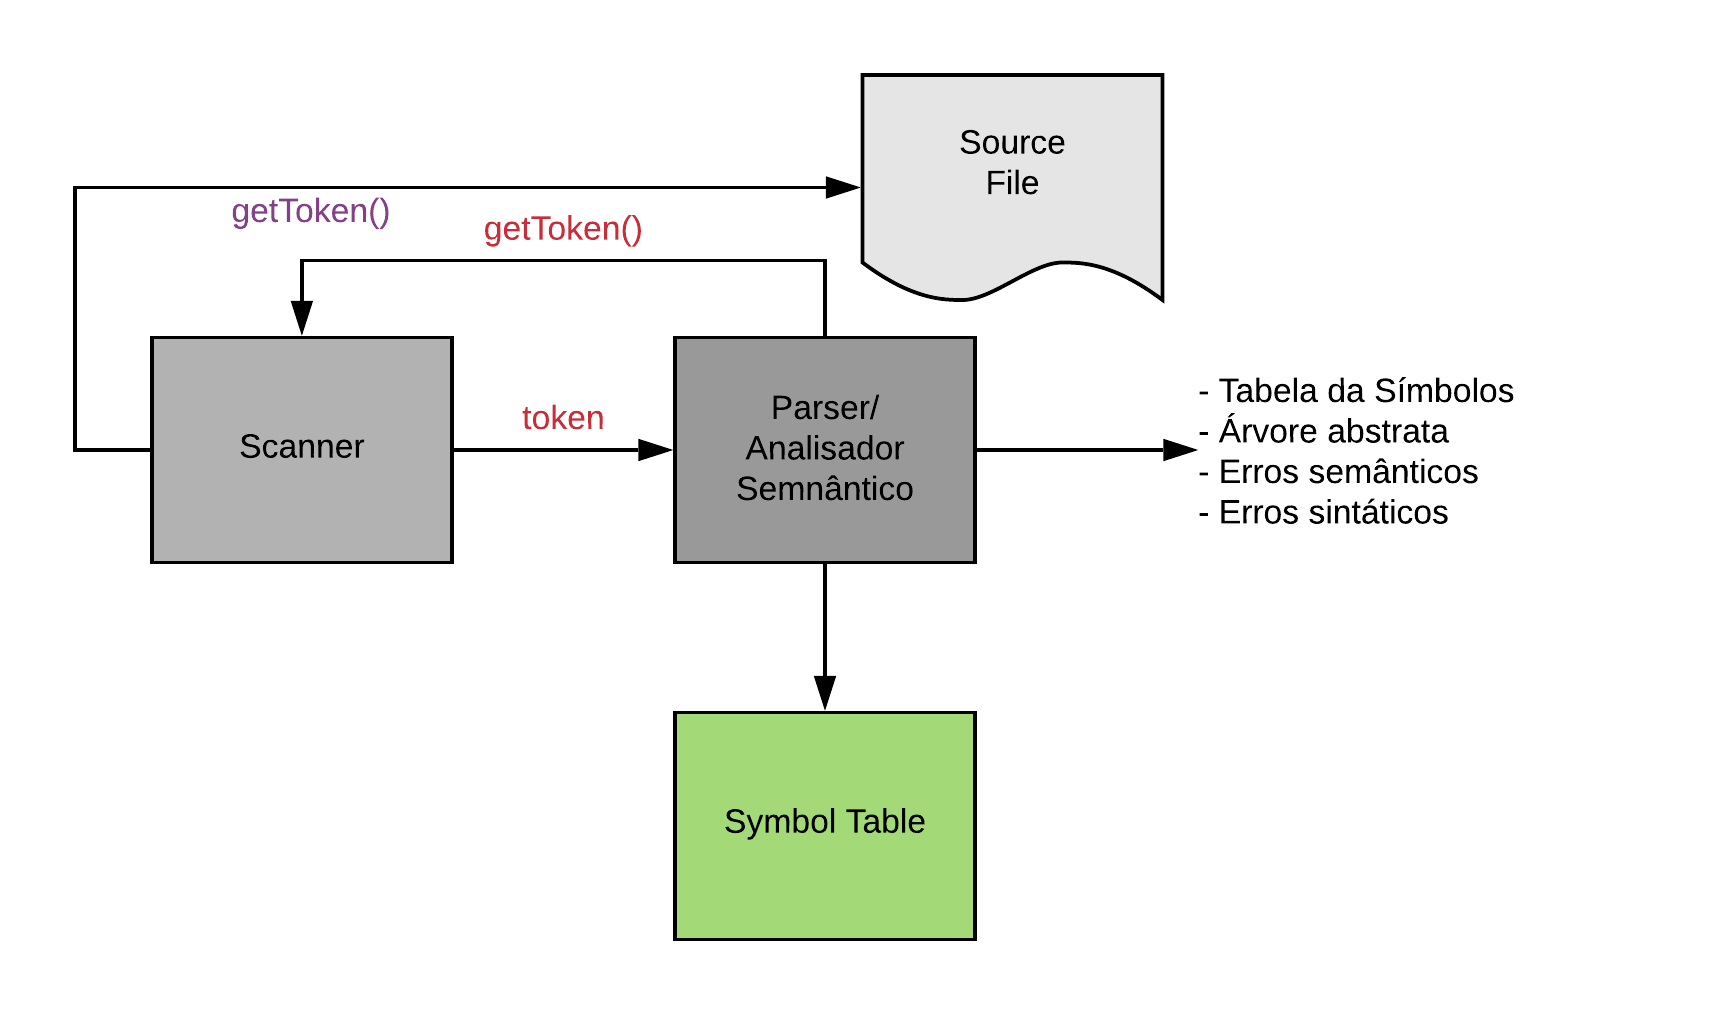
\includegraphics[scale=0.8]{img/diagrama-tradutores.png}
\end{figure}

O programa começa pela execução do módulo de análise, o qual imediatamente chama o scanner como co-rotina, e este retorna um \it{token} para o analisador. O analisador por sua vez vez decide entre
imediatamente pedir outro token, executar alguma redução ou realizar ações semânticas. É neste módulo que os identificadores são inseridos na tabela
de símbolos e realizada a ligação entre os nós da árvore correspondentes a identificadores e suas respectivas entradas da tabela de símbolos. Este
ciclo se repete até que o scanner atinja fim de arquivo ou ocorra algum erro durante montagem da árvore sintática por conta do recebimento de
token inesperado. Caso o arquivo seja sintaticamente correto, ao final do programa é exibida a árvore abstrata relativa ao código fonte. Caso
haja erros/"imprecisões" semânticas (imprecisão seria por exemplo uma atribuição cujos tipos não batem), mensagens são exibidas também na saída padrão do console. Vale ressaltar que erros semânticos \bf{não impedem a geração da árvore abstrata}, mas podem gerar \bf{inconsistências} nela e na tabela de símbolos.

Ao final da execução do programa, são exibidas a árvore abstrata produzida e em seguida a tabela de símbolos.

\subsection{Tratamento de Erros}

\subsubsection{Sintático}
O analisador produzido reporta alguns erros comuns, quais sejam:

\begin{itemize}{
		\item não inserção de ponto e vírgula após o valor a ser retornado pelo \IT{return} e o não fechamento de parêntese 
		\item expressão vazia (não são permitidas expressões lugal algum)
		\item não inserção de parêntese direito relativo à condição do \IT{if}
	}
\end{itemize}
Em caso de outros erros, a análise simplesmente é abortada. Em caso dos erros acima, a árvore sintática é montada naturalmente pelo \IT{bison}, embora fique inconsistente.

\subsection {Dificuldades Encontradas}

\subsubsection{Sintático}
\label{difSintatico}
Embora esta fase seja relativa ao analisador semântico, faz-se necessário um relato das dificuldades encontradas no desenvolvimento do analisador sintático pois, conforme dito em \ref{implementacao},
o analisador foi completamente refeito. Nesta nova implementação, as dificuldades principais, não houve muitas dificuldades, pois que já se sabia como lidar com a maioria as que surgiram. Um dos obstáculos encontrados foi quanto à decisão sobre quais tokens  ou cabeças de regras deveriam possuir seus próprios nós na árvore, visto que algumas produções são \it{dummy} e identificadores certamente requerem um nó para cada, além claro de uma conexão com sua respectiva entrada na tabela de símbolos. Foi também encontrada dificuldade a respeito de quais campos deveriam estar presente na estrutura de dados que forma cada nó da árvore abstrata e sobre quais regras podiam de fato ser tratadas como \it{dummy}.

Não houve problemas acerca da montagem da árvore de maneira geral, a menos do encadeamento da lista de parâmetros; durante certa etapa do desenvolvimento, houve dúvidas sobre como proceder no encadeamento da lista de parâmetros. Ao final, optou-se por cada parâmetro fazer parte de uma lista encadeada simples cujos elementos eram todos do mesmo tipo (tipo \it{No}), porém não diretamente faziam parte da árvore.

\subsubsection{Semântico}
\label{semantico}

Certamente a maior dificuldade enfrentada nessa fase foi a não percepção de todos os possíveis erros semânticos passíveis de ocorrência. Essa situação causou a imprevisibilidade do tempo necessário à conclusão do projeto, bem como consecutivos tropeços por não ter implementado a estrutura \it{No} com isso em mente. Dito isto, algumas das dificuldades superadas ao longo da realização desta fase foram:
\begin{itemize}
	\item resolução de escopo: como assegurar que parâmetros tinham como contexto a função à que pertenciam 
	\item lista de parâmetros/argumentos: qual a melhor maneira de encadeá-los
	\item lista de argumentos: como saber se uma função é chamada com argumentos cujos tipos batem com a assinatura da função
	\item resolução de escopo: melhor forma de diferenciar os escopos (em termos de eficiência, uma função \it{hash} seria a melhor opção; porém, a fim de simplificar a implementação, é feito por meio da comparação de caracteres)
\end{itemize}
Além dessas dificuldades relacionadas especificamente à análise semântica, registre-se que a maior parte do prazo de três semanas e 3 dias para esta entrega foi gasto refazendo a gramática, entendendo melhor o funcionamento do \it{bison} e criando as estruturas de dados a serem usadas na contrução da AST de modo a minimizar os \it{leaks} de memória. Também, fatores externos à disciplina (entregas de outras disciplinas) influenciaram bastante negativamente a qualidade da entrega.

Não foi possível implementar \it{tudo} que a análise semântica deveria fazer; isso deve ser feito para a próxima entrega e relatado juntamente com ela.

\subsection{Arquivos de teste}
Os arquivos de teste encontram-se na nos subdiretórios da pasta \href{https://github.com/maffei2443/unb_tradutores/tree/new_master/trab4/test}{\IT{test}} . Cada subdiretório contém os arquivos de teste relativos à cada fase do trabalho (léxico, sintático e semântico). A seguir, lista-se as pastas e descreve-se as peculiaridades de organização de cada uma:
\begin{itemize}
	\item léxico: contém arquivos com prefixo \it{c} ou \it{e}, os quais estão respectivamente corretos ou errados para o léxico, respectivamente
	\item sintático: organização idêntica à do léxico
	\item semântico: 
\end{itemize}

\section{Referências}
Foram utilizados basicamente os manuais do flex \cite{flex} e do bison \cite{bison}, além da documentação do cabeçalho \it{uthash} \cite{uthash}
Tais fontes não são de fácil compreensão, o que demandou esforços consideráveis em algumas situações.
% ---
% Finaliza a parte no bookmark do PDF, para que se inicie o bookmark na raiz
% ---
\bookmarksetup{startatroot}% 
% ---

% ---
% Conclusão
% ---
\postextual

\bibliography{bib}

\end{document}
